\documentclass[a4paper,abstracton]{scrreprt}
\usepackage[T1]{fontenc}
\usepackage[utf8]{inputenc}
\usepackage[ngerman]{babel}
\usepackage{pdfpages} 

%correct linebreaking in bibliography
\usepackage{hyperref}
\usepackage{breakurl}

%lists
\usepackage{mdwlist}

%pictures
\usepackage{float}
\usepackage{graphicx}
\graphicspath{{img/}}

%biblatex
\usepackage[babel,german=quotes]{csquotes}
\usepackage[style=authortitle]{biblatex}
%\bibliography{bib}
\bibliography{test}
\defbibheading{lit}{\chapter{Literaturverzeichnis}}
\setlength\bibitemsep{2\itemsep}
\usepackage{filecontents}

\begin{filecontents}{test.bib}
@Electronic{entoloma,
  Title                    = {Roetlinge / Entoloma},
  Author                   = {Machiel Evert Noordeloos},
  Url                      = {http://www.entoloma.nl/html/duits.html},
  Keywords                 = {entoloma},
  Note                     = {Navigation: Deutsch, Rötlinge},
  Owner                    = {Kevin},
  Urldate				   = {2014-07-03}
}
@Electronic{faktenuber,
  Title                    = {Fakten über Rötlinge},
  Author                   = {fakten-uber.de},
  Url                      = {http://fakten-uber.de/rötlinge},
  Keywords                 = {faktenuber},
  Note                     = {Navigation: Suche, Rötlinge},
  Owner                    = {Kevin},
  Urldate				   = {2014-07-03}
}
@Electronic{beschreibung,
  Title                    = {Rötling, Entoloma},
  Author                   = {R. Winkler},
  Url                      = {http://www.pilze.ch/pilzbestimmung/artenlisten/Entoloma.htm},
  Note                     = {Navigation: Pilzbestimmung, Gattungen und Arten, Entoloma},
  Keywords                 = {beschreibung},
  Owner                    = {Kevin},
  Urldate				   = {2014-07-03}
}
@Electronic{schildroetling,
  Title                    = {Steckbrief zu: Entoloma clypeatum},
  Author                   = {Fredis-Pilzseite.de},
  Url                      = {http://www.fredis-pilzseite.de/entoloma-clypeatum-1/},
  Keywords                 = {schildroetling},
  Owner                    = {Kevin},
  Urldate				   = {2014-07-03}
}
@Electronic{scherbengelb,
  Title                    = {Scherbengelber Rötling - Entoloma cetratum},
  Author                   = {123pilze.de},
  Url                      = {http://www.123pilze.de/DreamHC/Download/ScherbengelberRoetling.htm},
  Keywords                 = {scherbengelb},
  Note                     = {Navigation: Pilze nach Alphabet geordnet, Pilze alphabetisch geordnet, Scherbengelber Roetling},
  Owner                    = {Kevin},
  Urldate				   = {2014-07-03}
}
@Electronic{riesenroetling,
  Title                    = {Riesenroetling - Entoloma sinuatum},
  Author                   = {pilzfotopage.de},
  Url                      = {http://www.pilzfotopage.de/Agaricales/slides/Entoloma_sinuatum.html},
  Keywords                 = {riesenroetling},
  Note                     = {Navigation: Agaricales, Entoloma sinuatum},
  Owner                    = {Kevin},
  Urldate				   = {2014-07-03}
}
@Electronic{russblaettrig,
  Title                    = {Rußblättriger Rötling - Entoloma jubatum},
  Author                   = {tintling.com},
  Url                      = {http://tintling.com/pilzbuch/arten/e/Entoloma_jubatum.html},
  Keywords                 = {russblaettrig},
  Note                     = {Navigation: Pilzbuch, Artenindex, Entoloma jubatum},
  Owner                    = {Kevin},
  Urldate				   = {2014-07-03}
}
@Electronic{stahlblau,
  Title                    = {Stahlblauer Rötling - Entoloma nitidum},
  Author                   = {tintling.com},
  Url                      = {http://tintling.com/pilzbuch/arten/e/Entoloma_nitidum.html},
  Keywords                 = {stahlblau},
  Note                     = {Navigation: Pilzbuch, Artenindex, Entoloma nitidum},
  Owner                    = {Kevin},
  Urldate				   = {2014-07-03}
}
@Book{kosmos,
  Title                    = {Der Kosmos-Pilzatlas},
  Author                   = {Roger Phillips},
  Publisher                = {Franck-Kosmos Verlag},
  Year                     = {1990},
  Edition                  = {2},

  Owner                    = {Kevin},
  Timestamp                = {2014.07.03}
}
@Book{naturfuehrer,
  Title                    = {Pilze, sicher bestimmen mit Foto und Zeichnung},
  Author                   = {Karin Montag},
  Publisher                = {Franck-Kosmos Verlag},
  Year                     = {2003},
  Edition                  = {2},

  Owner                    = {Kevin},
  Timestamp                = {2014.07.03}
}


\end{filecontents}

%table 
\usepackage{pbox}
\usepackage{booktabs}

%set numeration depth
\setcounter{secnumdepth}{3}
%set how many numbers show up in table-of-contents
\setcounter{tocdepth}{2}

\begin{document}
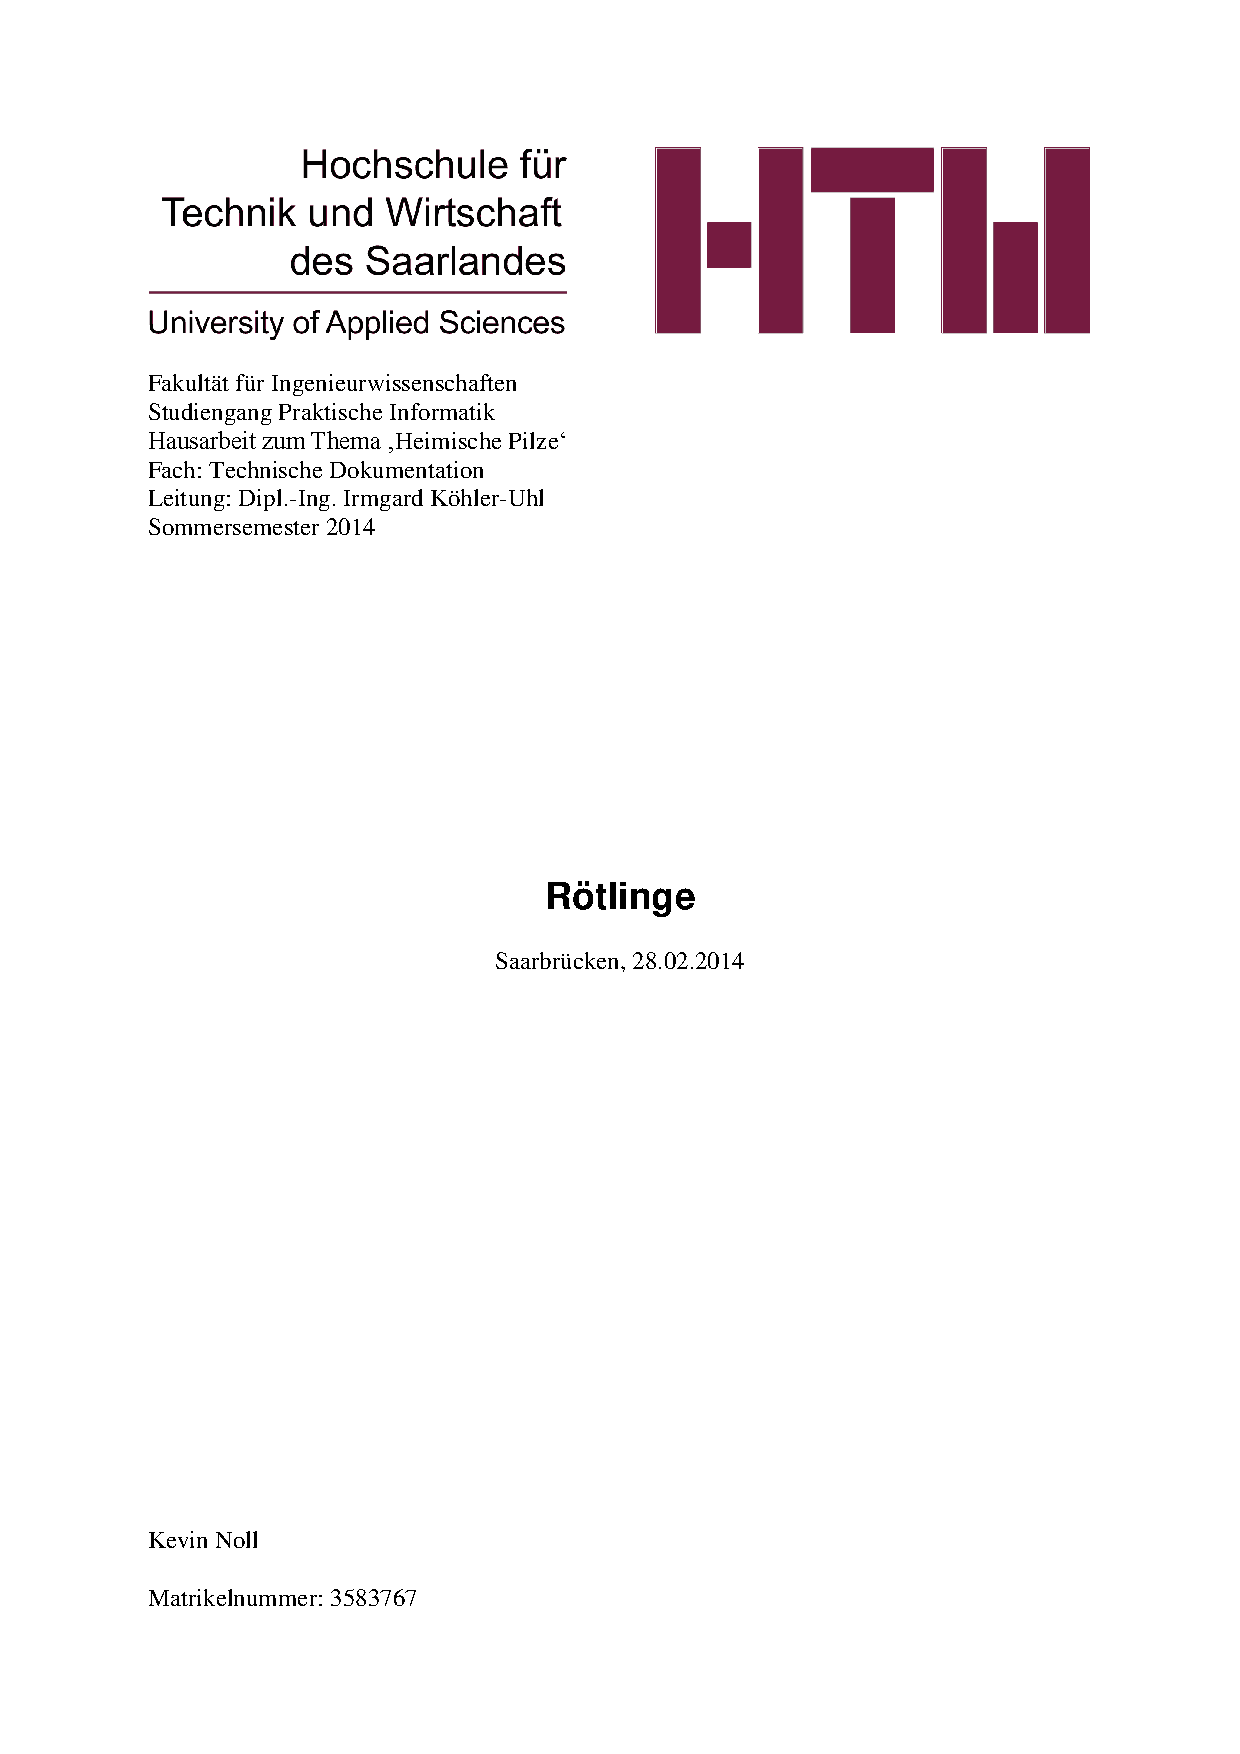
\includepdf[]{deckblatt.pdf}

%\author{Kevin Noll}
%\subject{Pilze und so}
%\title{Roetlinge, yo}
%\publishers{htwsaar}
%\maketitle
\tableofcontents
\listoffigures
%\listoftables

\begin{abstract}
\begin{quote}%abstand rechts und links
Diese Arbeit befasst sich mit der Beschreibung einer Pilzgattung in der Ordnung der Champignonartigen, in der Familie der Rötlingsverwandten. Es handelt sich dabei um die sogenannten \emph{Rötlinge -- lateinisch Entoloma --}.
\end{quote} 
\end{abstract}

\chapter{Vorwort}
Diese Ausarbeitung ist Bestandteil einer Reihe von Ausarbeitungen, die im Zuge der Vorlesung "'Technische Dokumentation"' entstanden sind. Der Kerngedanke bei der Anfertigung dieser Arbeit ist, zu erlernen, wie man mit fachbezogenen Texten umgeht -- von der Recherche über die Erstellung bis hin zur Anfertigung eines korrekten Literaturverzeichnisses. Unter dem Schirmthema \emph{Heimische Pilze} beschäftigt sich diese Ausarbeitung mit den Rötlingen (lat.: "'Entoloma"'). Es werden unter anderem Kenntnisse über Allgemeinheiten, das Vorkommen, die Beschreibung des Pilzes sowie die bei Pilzen so wichtigen Verwechslungsmöglichkeiten vermittelt. Weiterhin wird eine Auswahl ausgesuchter Arten einzeln betrachtet.
\chapter{Rötlinge}
\section{Allgemeines}
Rötlinge (lat.: "'Entoloma"') sind eine direkte Untergruppe -- auch Gattung genannt -- der Familie der Rötlingsverwandten (lat.: "'Entolomataceae"'). Wie alle Arten der Rötlingsverwandten besitzen die Rötlinge rosa- bis braunfarbenes Sporenpulver. Die Sporen der Rötlinge sind dabei im Gegensatz zu vielen anderen Gattungen der Familie eckig, was jedoch nur unter einem Mikroskop ersichtlich ist. Weiterhin besitzen viele Arten der Rötlinge sogenannte Zystiden. \footcite{entoloma}

Allgemein sind fast alle Rötlingsarten entweder ungenießbar oder sogar giftig. Giftige Arten sollten weder eingesammelt noch zubereitet werden. Die wenigen Arten welche nicht giftig sollten jedoch ebenfalls gemieden werden, da sehr leicht verwechselbar mit anderen giftigen Arten. \footcite{kosmos}

\section{Vorkommen}
Da die Rötlinge eine ausgesprochen große Gattung darstellen kommen sie an unterschiedlichsten Orten mit unterschiedlichsten Bedingungen vor. Auch können diese nicht auf eine Jahreszeit begrenzt werden da unterschiedliche Arten zu unterschiedlichen Zeiten im Jahr vorkommen. Während der \emph{Schildrötling -- Entoloma clypeatum --} beispielsweise hauptsächlich im Frühling unter Obstbäumen, Schlehen und Weißdorn (Rosengewächse) vorkommt, findet man den \emph{Sternsporigen Rötling -- Entoloma conferendum --} hauptsächlich von Juni bis Oktober auf Magerwiesen und wenig gedüngten Weiden. Der \emph{Frühlingsglöckling -- Entoloma vernum --} wächst normalerweise im Frühling bei Nadelbäumen oder an grasigen Stellen. \footcite{naturfuehrer} 

Allgemein können Rötlinge in Wäldern, Wiesen und Mooren bis in die alpine Stufe gefunden werden. Die meisten Arten leben dabei im Boden, jedoch gibt es auch einige wenige Arten die Totholz zersetzen oder an Bäumen leben. \footcite{faktenuber}

\section{Beschreibung}
Rötlinge kommen mit kleinen bis großen Fruchtkörpern in vielen verschiedenen Farben und Formen vor. Die Formen des Hutes der Rötlinge reichen von glockig-kebelig über breitgebuckelt, gewölbt, mit oder ohne Papille bis zu genabelt oder trichterig. Die Farbe des Fruchtkörpers kann dabei unterschiedlichster Art sein, erscheint jedoch meist in grauen bis braunen Tönen von blass bis sehr dunkel. Manche Gattungsanhänger bilden jedoch auch intensive Blautöne aus, selten können auch Grüntöne oder Rosatöne gefunden werden. 

Die Oberfläche des Pilzhutes ist im Normalfall metallisch glänzend, in selteneren Fällen jedoch auch filzig, faserig oder etwas schuppig. die Lamellen sind durch das bereits erwähnte rosafarbene Sporenpulver dementsprechend gefärbt. Dies ist besonders bei hell gefärbten Lamellen gut zu beobachten.
\footcite{beschreibung}

\section{Versuch der Aufteilung in mehrere Gattungen}
Aufgrund der größe dieser Gattung wurde bereits versucht diese in mehrere Untergattungen aufzuteilen. Dabei weisen besonders die deutschen Namen der Arten auf diese Gruppierungen hin. Diese lassen sich grob unterteilen in:
\begin{itemize}
\item \emph{Glöcklinge (Nolanea)} für dünnfleischige Arten mit gewölbtem, gebuckeltem bis glockigem Hut.
\item \emph{Zärtlinge (Leptiona)} für zartfleischige Arten mit niedergedrückter bis genabelter Hutform.
\item \emph{die eigentlichen Rötlinge (Entoloma, Rhodophyllus)} für Arten mit etwas fleischigeren bis dickfleischigen Fruchtkörpern mit breitkegelig-gewölbtem Hut und teilweise starkem Mehlgeruch.
\item \emph{Nabelrötlinge (Eccilia)} mit exzentrischem bis seitlichem Stiel und herablaufenden Lamellen.
\end{itemize}
\footcite{beschreibung}

\section{Verwechslungsmöglichkeiten}
Die meisten Rötlingsarten sehen ihren Artgenossen sehr ähnlich. Viele Rötlings sind sogar mit bloßem Auge nicht unterscheidbar und lediglich mit Hilfe eines Mikroskops korrekt zuzuordnen. Dies macht es speziell für Pilzsammler gefährlich, da beliebte Speisepilze wie der Schildrötling (Siehe~\ref{ref:schildroet}) sehr leicht mit anderen Rötlingsarten verwechselt werden können, teilweise mit fatalen Folgen. Wer sich also nicht sehr genau mit den Merkmalen der Rötlinge auskennt sollte im Zweifel einen Experten zu Rate ziehen, oder den Pilz erst gar nicht einsammeln.
\section{Geniessbarkeit}
Innerhalb der Familie der Rötlinge gibt es bis auf wenige Ausnahmen lediglich ungenießbare Arten. Einige davon sind sogar giftig und seltene sogar sehr giftig. Eine Ausnahme ist beispielsweise der Schildrötling, welcher als beliebter Speisepilz gezählt werden kann. 
\section{Unterarten}
\subsection{Übersicht}
Eine Auswahl der verschiedenen Arten von Rötlingen kann folgender Tabelle entnommen werden.


\bigskip
\begin{tabular}{cccc}
\toprule
\parbox{2cm}{\centering Deutscher Name} & \parbox{2cm}{\centering Botanischer Name} & \parbox{6cm}{\centering Vorkommen} & \parbox{2cm}{\centering Speisewert} \\
\midrule
\parbox{2cm}{\centering Grosssporiger Zärtling} & \parbox{2cm}{\centering Entoloma aethiops} & \parbox{6cm}{ auf Wiese, am Waldrand, vorwiegend auf kalkhaltigem Boden bis in höhere Lagen; Sommer bis Herbst.} & \parbox{2cm}{\centering kein Speisepilz} \\
\addlinespace[0.4cm]
\parbox{2cm}{\centering Schwarz-schneidiger Rötling} & \parbox{2cm}{\centering Entoloma caesiocinctum} & \parbox{6cm}{im Moor, bei Torfmoos (Sphagnum); Sommer bis Herbst} & \parbox{2cm}{\centering giftig } \\
\addlinespace[0.4cm]
\parbox{2cm}{\centering Nutzloser Glöckling} & \parbox{2cm}{\centering Entoloma inutile} & \parbox{6cm}{in Trockenrasen, Waldlichtungen, Heide, auf saurem Boden; Sommer bis Herbst} & \parbox{2cm}{\centering kein Speisepilz } \\
\addlinespace[0.4cm]
\parbox{2cm}{\centering Blassbrauner Schlehenrötling} & \parbox{2cm}{\centering Entoloma saepium} & \parbox{6cm}{bei Rosenblütengewächsen (Weissdorn, Schlehen usw.); Frühling bis Sommer} & \parbox{2cm}{\centering essbar } \\
\addlinespace[0.4cm]
\parbox{2cm}{\centering Heiderötling} & \parbox{2cm}{\centering Entoloma elodes} & \parbox{6cm}{zwischen Torfmoos (Sphagnum); Sommer bis Herbst} & \parbox{2cm}{\centering kein Speisepilz } \\
\bottomrule
\end{tabular}

\footcite{beschreibung}
\bigskip

Größere Bedeutung kommt folgenden Exemplaren der Rötlinge zu, weshalb diese genauer betrachtet werden:
\subsection{Riesenrötling -- Entoloma sinuatum}
Der Riesenrötling ist in ganz Deutschland zu finden, bevorzugt jedoch in lichten Laubwäldern, besonders nahe Buchen-, Tannen und Eichenbäumen. Der Pilz ist stark giftig und kann Todesfälle verursachen, weshalb er von Speisepilzsammlern gemieden werden sollte. Er ist leicht zu verwechseln mit dem essbaren Mairitterling sowie dem nebelgrauen Trichterling.

Folgen des Verzehrs sind unter anderem Reizungen der gastrointestinalen Schleimhäute, was heftige Durchfälle und Erbrechen auslöst sowie zu heftigen Bauchschmerzen, Koliken, Krämpfen und Schockzuständen führt. Das injizierte Gift sowie die Giftmenge ist weitestgehend unbekannt, jedoch sind ältere Menschen und Kinder besonders gefährdet. Zirka 40\% aller Pilzvergiftungen werden durch den Riesenrötling verursacht.
\footcite{riesenroetling}

\begin{figure}[H]
\centering
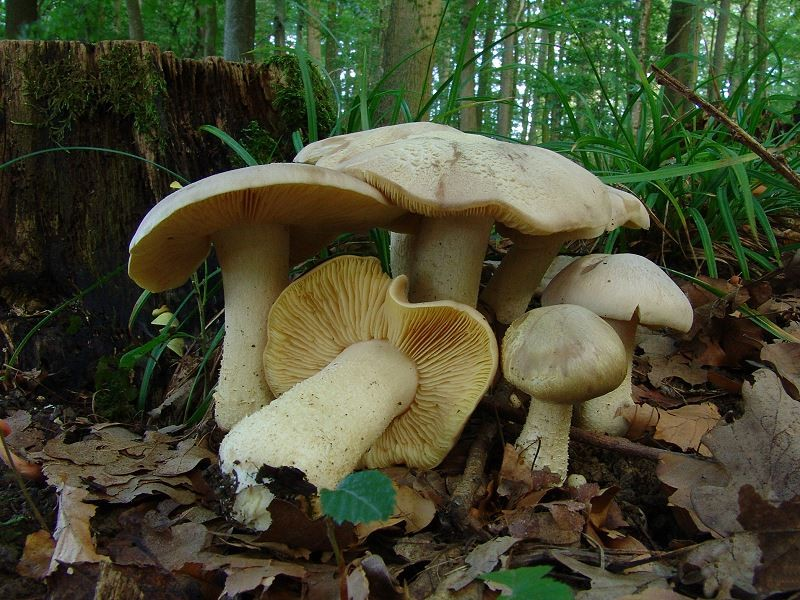
\includegraphics[scale=0.2]{riesenroetling}
\caption{der Riesenrötling -- Entoloma sinuatum }
\label{fig:riesenroetling}
\end{figure}

\subsection{Schildrötling -- Entoloma clypeatum}
\label{ref:schildroet}
Der Schildrötling kommt in ganz Deutschland vor, jedoch nirgends gehäuft. Er kann hauptsächlich unter Schlehen- sowie Weißdorngebüschen gefunden werden, sowie an Weg- und Waldrändern, aber auch auf Wiesen und in Hecken als auch in Park- und Gartenanlagen. Meistens werden Gruppen von Pilzen gefunden, alleinstehende Exemplare sind eher selten. 

Auch von Experten wird der Schildrötling häufig verwechselt mit dem April-Rötling, da sich auch makroskopisch nur kleine Unterschiede zu diesem feststellen lassen.

Der Schildrötling ist ein guter Speisepilz, dennoch sollten sie von Sammlern die diese Pilzart nicht genau kennen vermieden werden, da sie ihren ungenießbaren und teilweise sogar stark giftigen Rötlingsverwandten zum verwechseln ähnlich sehen.
\footcite{schildroetling}

\begin{figure}[H]
\centering
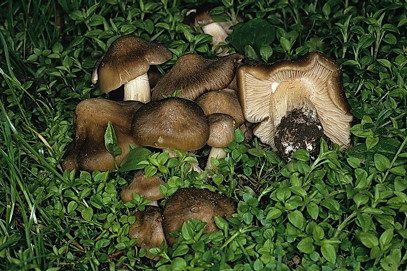
\includegraphics[scale=22]{schildroetling}
\caption{der Schildrötling -- Entoloma clypeatum }
\label{fig:schildroetling}
\end{figure}

\subsection{Rußblättriger Rötling -- Entoloma jubatum}
Der rußblättrige Rötling ist ebenfalls weit verbreitet, jedoch nicht sehr häufig. Er kann hauptsächlich vereinzelt oder in kleinen Gruppen auf ungedüngten Wiesen gefunden werden. Er hat einen bis zu Hut mit bis zu 6 cm Durchmesser und ist bis zu 12 cm hoch. Markant ist der lange, dünne Fuß des Pilzes. Weiterhin hat er einen unauffälligen Geruch, und einen sehr bitteren Geschmack, weshalb er sich nicht als Speisepilz eignet.
\footcite{russblaettrig}
\begin{figure}[H]
\centering
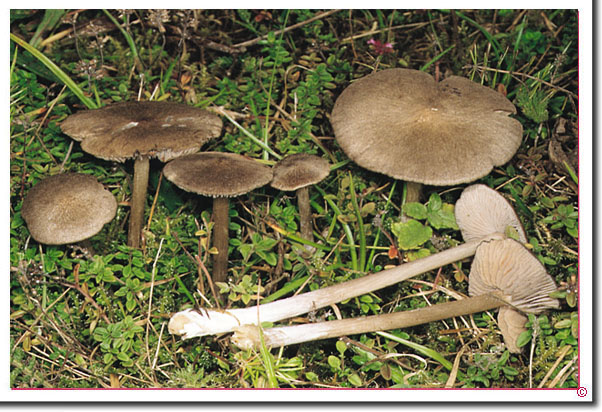
\includegraphics[scale=0.3]{russblaettrig}
\caption{der Rußblättrige Rötling -- Entoloma jubatum }
\label{fig:russblaettrig}
\end{figure}

\subsection{Scherbengelber Rötling}
Scherbengelbe Rötlinge sind vor allem im Nadelwald, in der Heide, in Wiesen sowie auf saurem Boden zu finden. Die Jahreszeiten des Pilzes reichen vom Frühsommer bis in den Herbst. Die Lamellen des Hutes sind lange weiß bis gelblich, später dann rosa bis rotbraun. Der Hut ist meist graubraun, der Rand ist feucht durchscheinend. Weiterhin hat der Hut keinen Buckel. Der Stiel ist ähnlich gefärbt wie der Hut, sehr zerbrechlich und außerdem fein bepudert.
Der scherbengelbe Rötling ist auch als Scherbengelber Glöckling, Ockerblättriger Glöckling sowie als Ockerblättriger Rötling bekannt. Er ist giftig und deswegen nicht zum Verzehr geeignet. Wie viele seiner Artgenossen ist er nur unter dem Mikroskop eindeutig zu identifizieren.
\footcite{scherbengelb}
\begin{figure}[H]
\centering
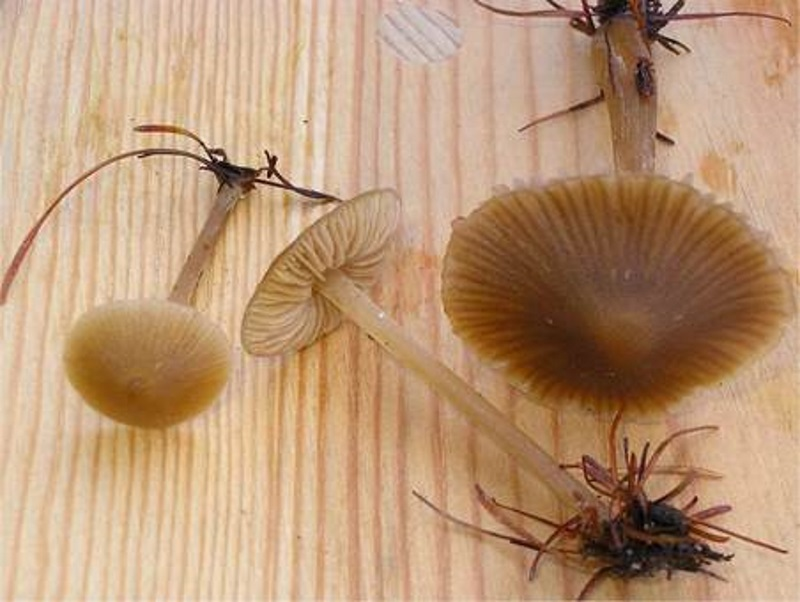
\includegraphics[scale=0.6]{scherbengelb}
\caption{der Scherbengelbe Rötling -- Entoloma cetratum }
\label{fig:scherbengelb}
\end{figure}

\subsection{Stahlblauer Rötling}
Der stahlblaue Rötling kommt hauptsächlich in sauren, moosigen, streng nährstoffarmen Fichtenforsten sowie in armen Mischwäldern mit Fichten vor. Außerdem kann er in Hochmooren sowie auf Torf gefunden werden. Im Tiefland mittlerweile fehlend, wird er auch in höheren Lagen kaum mehr gefunden.
Der Hut ist kegelig bis gewölbt und oft mit spitzem Buckel sowie stahlblau gefärbt, was dem Pilz seinen Namen verleiht. Die Lamellen sind im Gegensatz zur Oberseite des Huts weiß gefärbt. Der Stiel ist weiß bis ebenfalls stahlblau, sehr gebrechlich und langfaserig.

Stahlblaue Rötlinge sind sehr empfindlich gegen Düngung sowie Kalkung und Emissionen aus dem Straßenverkehr und der Industrie, weshalb er entsprechend selten geworden ist. Er steht deswegen auf der roten Liste. Weiterhin ist er giftig.
\footcite{stahlblau}
\begin{figure}[H]
\centering
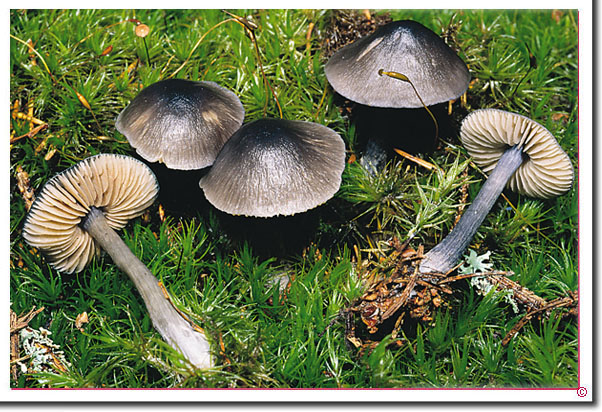
\includegraphics[scale=0.4]{stahlblau}
\caption{der Stahlblaue Rötling -- Entoloma nitidum }
\label{fig:stahlblau}
\end{figure}

\printbibliography[heading=lit]

\end{document}